\documentclass[../../main.tex]{subfiles}
\begin{document}
\begin{oframed}
  \subfile{problem}
\end{oframed}

{\bf [解答]}

$x^2+x+1=0$の2解は
\begin{align}
  \omega=\dfrac{-1+\sqrt{3}i}{2}, \bar{\omega} = \dfrac{-1-\sqrt{3}i}{2} = \omega^2 \label{eq:1}
\end{align}
である．この$\omega$は$\omega^2+\omega+1=0$および$\omega^3=1$を満たす．

\begin{figure}[htb]
  \centering
  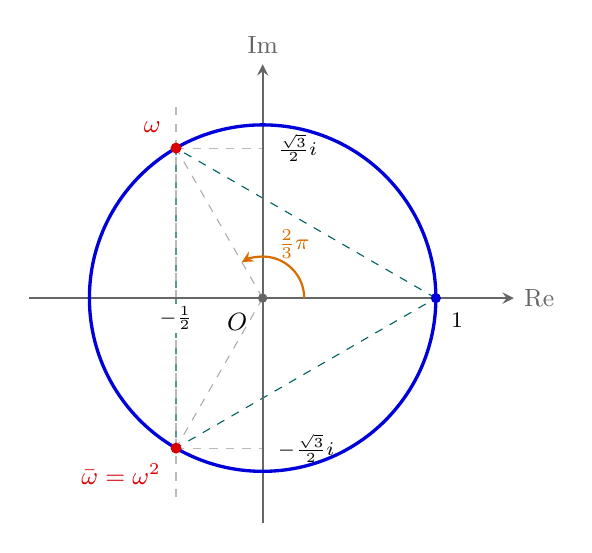
\begin{tikzpicture}[x=2.2cm, y=2.2cm, >=stealth, every node/.style={font=\small}]
    \coordinate (O) at (0,0);
    \coordinate (P0) at (1,0);
    \coordinate (W) at (120:1);
    \coordinate (Wbar) at (240:1);
    % 単位円と正三角形 1, omega, omega^2
    \draw[dashed, teal!75!black] (P0) -- (W) -- (Wbar) -- cycle;
    % 実部・虚部の射影線（破線）
    \draw[dashed, gray!55] (-0.5,-1.15) -- (-0.5,1.15);
    \draw[dashed, gray!55] (-0.5,0.866) -- (0,0.866);
    \draw[dashed, gray!55] (-0.5,-0.866) -- (0,-0.866);
    \draw[dashed, gray!65] (O) -- (W) (O) -- (Wbar);
    % 座標軸
    \draw[->, thick, gray!80!black] (-1.35,0) -- (1.45,0) node[right] {$\mathrm{Re}$};
    \draw[->, thick, gray!80!black] (0,-1.3) -- (0,1.35) node[above] {$\mathrm{Im}$};
    \draw[line width=1.2pt, blue!85!black] (O) circle[radius=1];
    % 偏角 2/3 pi
    \draw[orange!85!black, thick, ->] (0.24,0) arc[start angle=0, end angle=120, radius=0.24];
    \node[font=\footnotesize, orange!85!black] at (60:0.36) {$\frac{2}{3}\pi$};
    % 各点
    \node[circle, fill=gray!80!black, inner sep=1.2pt] at (O) {};
    \node[circle, fill=blue!85!black, inner sep=1.3pt] at (P0) {};
    \node[circle, fill=red!85!black, inner sep=1.4pt] at (W) {};
    \node[circle, fill=red!85!black, inner sep=1.4pt] at (Wbar) {};
    % ラベル
    \node[above left=2pt, red!85!black] at (W) {$\omega$};
    \node[below left=2pt, red!85!black] at (Wbar) {$\bar{\omega}=\omega^2$};
    \node[below right=2pt, font=\footnotesize] at (P0) {$1$};
    \node[below left=2pt] at (O) {$O$};
    \node[below=2pt, font=\scriptsize, fill=white, inner sep=1pt] at (-0.5,0) {$-\frac{1}{2}$};
    \node[right=2pt, font=\scriptsize] at (0,0.866) {$\frac{\sqrt{3}}{2}i$};
    \node[right=2pt, font=\scriptsize] at (0,-0.866) {$-\frac{\sqrt{3}}{2}i$};
  \end{tikzpicture}
  \caption{複素数平面上の単位円と$1$の虚数3乗根$\omega,\ \bar{\omega}=\omega^2$}
  \label{fig:cube_roots_of_unity}
\end{figure}

題意の式
\begin{align}
  F(x)=(x^{100}+1)^{100}+(x^2+1)^{100}+1
\end{align}
として$x=\omega,\omega^2$を代入すると
\begin{align}
  F(\omega)
  &=(\omega+1)^{100}+(-\omega)^{100}+1\\
  &=(-\omega^2)^{100}+\omega+1\\
  &=\omega^2+\omega+1=0
\end{align}
および
\begin{align}
  F(\omega^2)&=(\omega^2+1)^{100}+(\omega+1)^{100}+1\\
  &=(-\omega)^{100}+(-\omega^2)^{100}+1\\
  &=\omega^2+\omega+1=0
\end{align}
だから，因数定理より$F(x)$は$(x-\omega)(x-\omega^2)=x^2+x+1$で割り切れる．\qed

\newpage

\end{document}
